

\subsection{DFA Coverage Example}
\label{sec:coverageexample}
Bug reports related to regular expressions abound. 
 A search for ``regex OR regular expression'' in GitHub yields over 555,000 issues, with 22\% of those still being open. 
 One in particular illustrates how coverage metrics on the DFA could have brought a particular bug to the developer's attention sooner. This bug report\footnote{\url{https://github.com/maven-nar/nar-maven-plugin/issues/228}} describes an issue with the regular expression \verb!\d+\.d+! in the NAR plugin for Maven. 
Figure~\ref{fig:bug} shows the DFA of this regular expression built using RE2~\cite{re2}, and we take this opportunity to describe the DFA notation used throughout this paper\footnote{The regular expression in the bug is triggered by {\tt Matcher.find()} with a ManyMatch DFA. For simplicity, we show the FullMatch DFA, a subgraph of the ManyMatch.}. 

Node~0 is the start-state, indicated by the incoming arrow. 
Nodes with double-circles are accept states, such as Node~4. 
Node~e is the error state, denoting a mismatch. 
The edges are labeled with transitions, often using syntactic sugar for ease of interpretation. 
The edge $\overrightarrow{01}$ is traversed when a digit from \verb!0-9! is read. 
If any other character is read at Node~0, (i.e., \verb!not 0-9!), edge $\overrightarrow{0e}$ is traversed. 
 There is a self-loop on Node~1 for digits \verb!0-9!. 
 If the period character is read from Node~1, then edge $\overrightarrow{12}$ is traversed. 
%If any other character is read (i.e., not `\verb!/!), then edge $\overrightarrow{21}$ is traversed to Node~1. Since Node~1 is an accept state, any other character read from Node~1 reaches the error state, Node~e.

In RE2, when reading an input string, byte~{\tt [256]}, is added as a text-end marker. %, to mark the end of processing. 
For example, the input string ``0.0'' is transformed to the byte stream {\tt [48 46 48 256]}, as {\tt [48]} is the byte for `0', {\tt [46]} is for `.', and {\tt [256]} marks the end of the string. Byte [256] is matched on edges  `\verb![0-256]!', `\verb!not 0-9!',  `\verb!not d!', or `\verb!any except 0-9 and .!'. 

%\todo{replace `[0-256]` in the DFA with `any`; I think it's best not to explain what 256 means at this point}

%\adh{I would delete this paragraph and simply go with the last paragraph: the issue is not testing one of the branches, our approach would have fixed that.  Therefore the problem we are talking about exists in the wild at least sometimes.}
%With the regular expression in Figure~\ref{fig:bug}, input ``/root'' is rejected when it should be accepted, traversing $0 \rightarrow 2 \rightarrow 1 \rightarrow e$. 
%The string ``///''  is accepted should actually be rejected, traversing $0 \rightarrow 2 \rightarrow 2 \rightarrow 2 \rightarrow 1$. This final transition from $2 \rightarrow 1$ occurs because the RE2 tool that built the DFA reads a final byte (byte [256], to be exact) following the last character in the input string to signify the end of processing. The same though would have occurred for ``/root'', except the error state was reached when the first `o' was read, thus no further input characters were processed. 
%and As a result, the urlPattern ``/*'' matches an empty url and does not match the normal url. 
%The traversed path of these three inputs are , , . 

\begin{figure}[t]
	\centering
	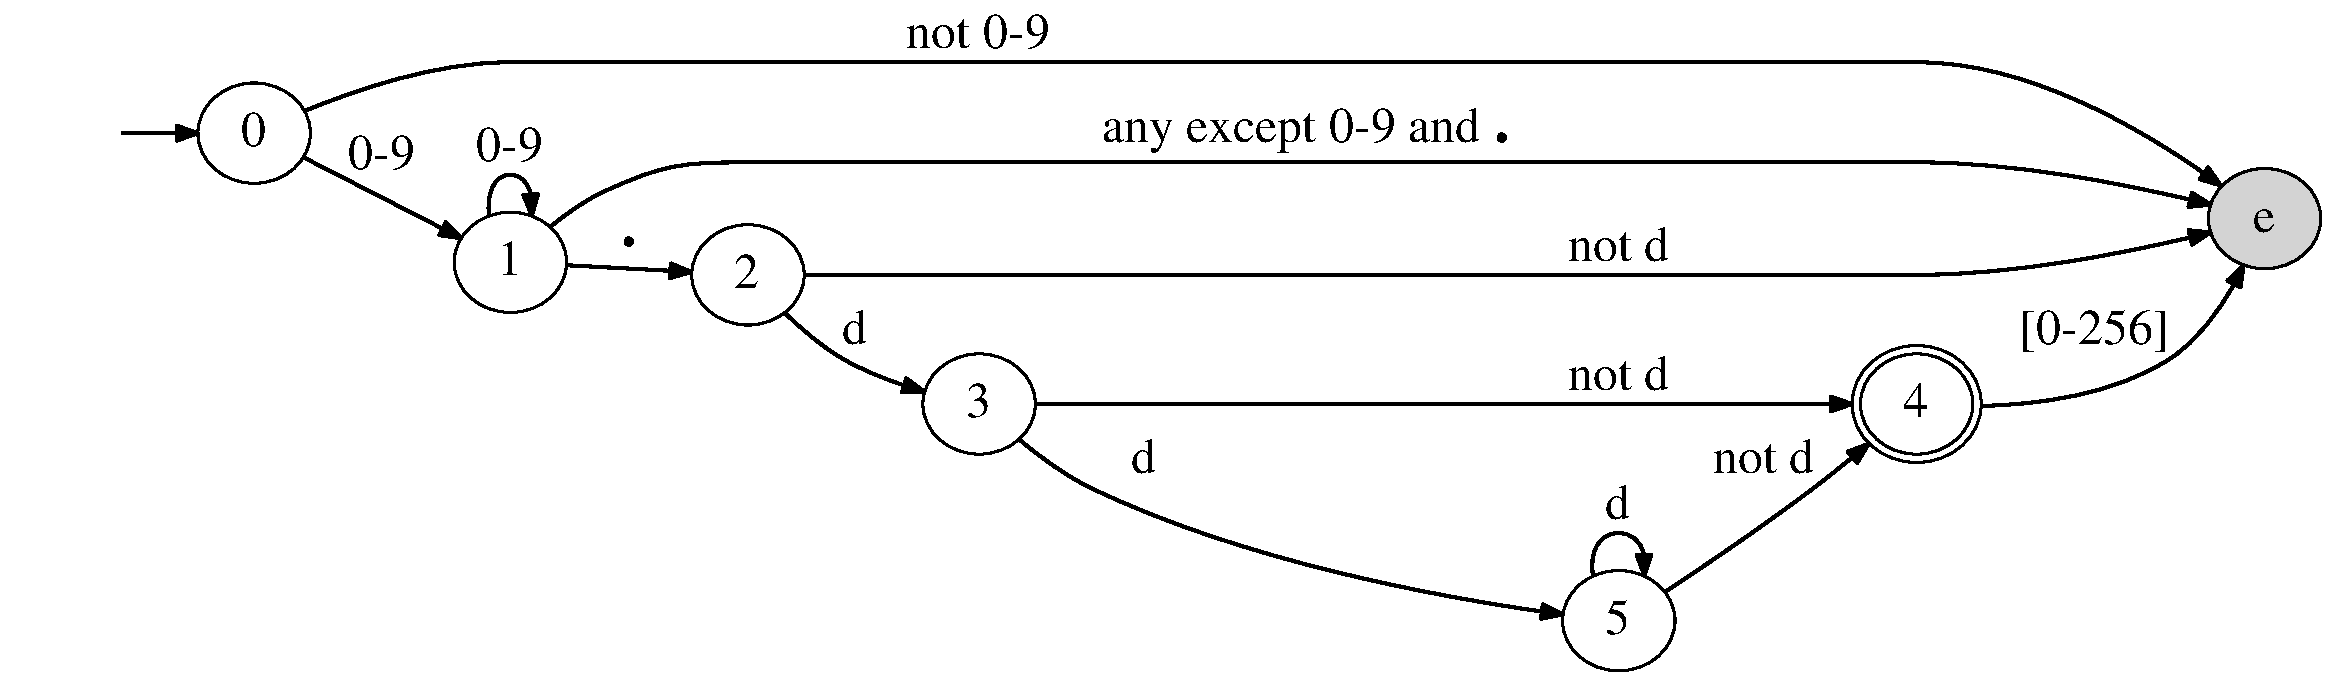
\includegraphics[width=0.48\textwidth]{figures/bug4}
	\vspace{-12pt}
	\caption{Full-match DFA for regular expression: {\tt \textbackslash d+\textbackslash .d+}}
	\label{fig:bug}    
	\vspace{-12pt}
\end{figure}

 The bug report mentions that the regular expression \verb!\d+\.d+! is buggy and the patch adds an escape before the second d, \verb!\d+\.\d+!. The intended behavior is to match input strings with one or more digits, followed by a period, followed by one or more digits.
 
In this work, the structural metrics could reveal this fault. 
With the DFA in Figure~\ref{fig:bug}, when Node~3 is reached, the fault may be revealed. 
Input "0.d" traverses $0 \rightarrow 1 \rightarrow 2 \rightarrow 3 \rightarrow 4$ and ends in an accept state, when it should fail. However, input "0.d3" traverses  $0 \rightarrow 1 \rightarrow 2 \rightarrow 3 \rightarrow 4 \rightarrow e$ and ends in an error state, as expected. 
Covering edge $\overrightarrow{2e}$ may also reveal the fault; input "2.3" traverses $0 \rightarrow 1 \rightarrow 2  \rightarrow e$ and ends in and error state, when it should be accepted.
Requiring coverage of all feasible nodes and edges could have revealed this fault in the regular expression. 

%That is, input "0" traverses $0 \rightarrow 1 \rightarrow e$, the expected behavior, and the fault is not revealed. 
%
%the problematic situation when the empty string ``'' is accepted while should be rejected. 
%The empty string is read as simply {\tt [256]}, traversing $\overrightarrow{01}$ to the accept state. 
%Without testing the empty string, the edge $\overrightarrow{01}$ would be uncovered.
%Presumably, in this case, failure to test the empty string led to a bug report. 
%%According to the bug report, the fix for this regular expression is to replace \verb!/*! with \verb!/.*+!, however, fixing the regular expression is not the goal of the work. 
%The goal of this work is to identify uncovered edges and nodes, such as $\overrightarrow{01}$. 
As with code coverage,  uncovered artifacts alert the programmer to untested behavior. Such coverage information can indicate that a regular expression is not well tested and for some inputs it may not behave as intended, as is the case here.

